\documentclass[11pt,a4paper]{article}
\usepackage[utf8]{inputenc}
\usepackage[spanish]{babel}
%\usepackage{amsmath}
%\usepackage{amsfonts}
%\usepackage{amssymb}
\usepackage{wrapfig}
\usepackage{float}
\usepackage{hyperref}
\usepackage[pdftex]{graphicx}
\usepackage{fancyhdr}
\usepackage[font=small,labelfont=bf]{caption}
\pagestyle{fancy}
\lhead{\bfseries Redes de Datos -- IPv6}
\rhead{}
%\chead{}
\newcommand{\HRule}{\rule{\linewidth}{0.5mm}}
\usepackage[left=2cm,right=2cm,top=2cm,bottom=2cm]{geometry}
\author{Ignacio Perez Laborda}

\renewcommand{\thefootnote}{\roman{footnote}}

\hypersetup{pdfborder = {0 0 0}}

\begin{document}

\begin{titlepage}

\begin{center}

% Upper part of the page

\includegraphics[width=0.25\textwidth]{./logo_UB.png}\\[1cm] 

\textsc{\LARGE Universidad de Belgrano}\\[1.5cm]

\textsc{\Large Redes De Datos}\\[0.5cm]

%title
\HRule \\[0.4cm]
{ \huge \bfseries Trabajo Practico 2 -- Cloud Computing}\\[0.4cm]
\HRule \\[1.5cm]

% Author and supervisor
\begin{minipage}{0.4\textwidth}
\begin{flushleft} \large
\emph{Alumno:}\\
Ignacio \textsc{P\'erez Laborda}\\
Barbara \textsc{Mart\'inez}\\
\end{flushleft}
\end{minipage}
\begin{minipage}{0.4\textwidth}
\begin{flushright} \large
\emph{Matricula:} \\
502--10426\\
502--10402\\
\end{flushright}
\end{minipage}\\[1.5cm]

\vfill

%Bottom of the page
{\large \today}

\end{center}

\end{titlepage}


\tableofcontents

\listoffigures

\newpage

\section{¿Que es IP?}
\subsection{Introducción Histórica}
En plena guerra fría para fines de los años sesenta, el Departamento de Defensa (DoD) norteamericano
necesitaba de un nuevo método para conectar sus distintos centros de investigación y centros 
gubernamentales y que además pueda ser extendida a otros medios de propagación. Esta responsabilidad 
cayo en manos de de ARPA(Advanced Research Projects Agency), la cual en la
reunión de la ACM de 1967 se diseño su estructura básica y se la nombro ARPANET. Para el año 
siguiente se realizaron las primeras adjudicaciones para la implementación de una red de conmutación
de paquetes con una velocidad de 50kbps\footnote{kilobits por segundo}. Dicha implementación fue
adjudicada a la recientemente creada BBN (Bolt Beranek and Newman), la cual fue creada para ese
propósito.\par
Para el año 1969 fue instalado el primer nodo de ARPANET en la Universidad de California en Los
Angeles seguida por los nodos de Stanford, Santa Barbara y la Universidad de Utah. Con estos cuatro
nodos se dio inicio a la red que al cabo de dos años ya se había expandido por todo USA y dos años
después cruzaría el atlántico para desembarcar en Europa.\par
Corriendo el año 1974 ARPANET ya necesitaba de un nuevo protocolo ya que el usado hasta el momento, 
llamado NCP (Network Control Protocol) mostraba muchas falencias al crecer tanto la red. La solución
vino de la mano de un paper que publico Vinton Cerf y Robert Kahn. Este protocolo fue el 
TCP(Transmission Control Protocol), pero este también se enfrento a ciertos problemas y 
restricciones.
\begin{wrapfigure}{r}{0.5\textwidth}
\centering
  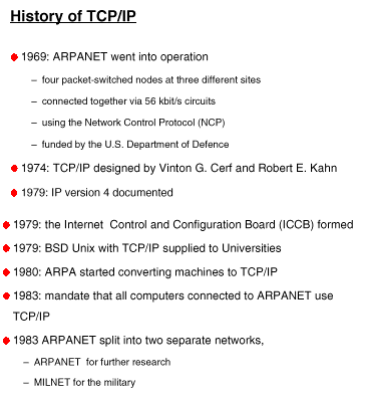
\includegraphics[width=0.48\textwidth]{historiaTCPIP.png}
 \caption[Historia de TCP/IP]{Linea temporal de TCP/IP}
\vspace{-15pt}
\end{wrapfigure}
Para el año 1978 se decidió dividir las responsabilidades entre un par de protocolos; el nuevo IP
(Internet Protocol) que se encargaría de enrutar los paquetes y comunicaciones de dispositivo a 
dispositivo, y TCP para la comunicación confiable de host a host. Aunque son dos protocolos que 
trabajan en capas distintas fueron pensados para operar en conjunto dentro de un conjunto, por eso
comúnmente se los denomina TCP/IP. La version actual, numero 4, del susodicho protocolo y de la cual
hablaremos mas adelante fue especificada en el año 1979.\par
Ya en la siguiente década ARPANET migro completamente a TCP/IP por mandato del Departamento de 
Defensa. En ese mismo año 1983 la red fue divida en dos ARPANET que siguió con su alcance original y
MILNET donde se desempeñarían las comunicaciones militares. Pero otra gran suceso de ese año fue la
inclusión del protocolo en el UNIX de la Universidad de Berkeley, el BSD 4.2.\par
Saltando tres años situándonos en 1986, la National Science Foundation construyo lo que serian los
cimientos de la internet que conocemos al financiar la construcción de una red para la conexión de
sus supercomputadoras. Esto gracias a la apertura de la NSF permitió a particulares conectarse a 
dicha red lo cual ayudo a su gran crecimiento, todo esto estaba y esta apoyado por el TCP/IP. Esta 
red existió hasta el año 1993, para ese entonces se era lo suficientemente maduro y rentable como 
para ser comercial y ya existían empresas dispuestas y con el conocimiento para llevarlo a cabo. Se 
puso en marcha un plan al año siguiente para reducir la influencia de la NFS y aumentar la 
rentabilidad de los incipientes ISP\footnote{Internet Service Provider} privados.\par
Mientras tanto el DoD y el gobierno norteamericano eligieron adoptar el modelo OSI y se pensó que
esto supondría el fin del modelo TCP/IP, incluso el gobierno llego a obligar su uso masivo, pero
TCP/IP siguió evolucionando sobre el fundamento de la practica y su calidad de estándar abierto.\par
Lo que nos puede dejar esta muy resumida historia del protocolo es que la internet no tiene un claro
inventor ni un destino claro, sino fue el trabajo en conjunto de varias personas e instituciones las
cuales querían solucionar sus problemas de comunicación. Fue gracias a las soluciones abiertas las
cuales permitió el mejoramiento por los usuarios, también los niveles de abstracción que se 
permitieron hizo realidad que varias tecnologías puedan convivir en armonía. Esta filosofía abierta
tan característica y que ha marcado tanto a la industria puede resumirse en el lema de la 
IETF\footnote{Internet Engineering Task Force}, expresado por David Clark: "Nosotros rechazamos 
reyes, presidentes y votaciones. Nosotros creemos en el consenso y en el código funcional".

\subsection{El Protocolo IP}
Este protocolo se encuentra en la segunda capa del modelo TCP/IP y la tercera del OSI. El se encarga
de transmitir los paquetes entre el origen y destino basándose en su dirección IP. Esto se logra
encapsulando los datos y formando su propio datagrama. Dentro se tienen dos partes principales el
encabezado y la carga, en el encabezado junto a otra metadata se coloca la dirección IP de origen y 
la de destino. El protocolo IP debe proveer de un servicio no orientado a la conexión no confiable y 
de mejor esfuerzo, también llamado servicio de datagramas. Esto quiere decir: no confiable, el 
protocolo no intenta recuperar los paquetes perdidos; no orientado a la conexión, cada paquete o 
datagrama es manejado independientemente IP desconoce si existe una secuencia lógica de envío; mejor
esfuerzo, IP no garantiza el servicio. Todo esto lleva a que otras capas se encarguen de la perdida
de los paquetes y solicitar su reenvío. IP también permite tres tipos de servicios: Unicast (uno a 
uno), Multicast (uno a varios) y Broadcast (uno a todos).\par
A continuación vemos la estructura de un datagrama de IP.
\begin{figure}[h!]
 \centering
 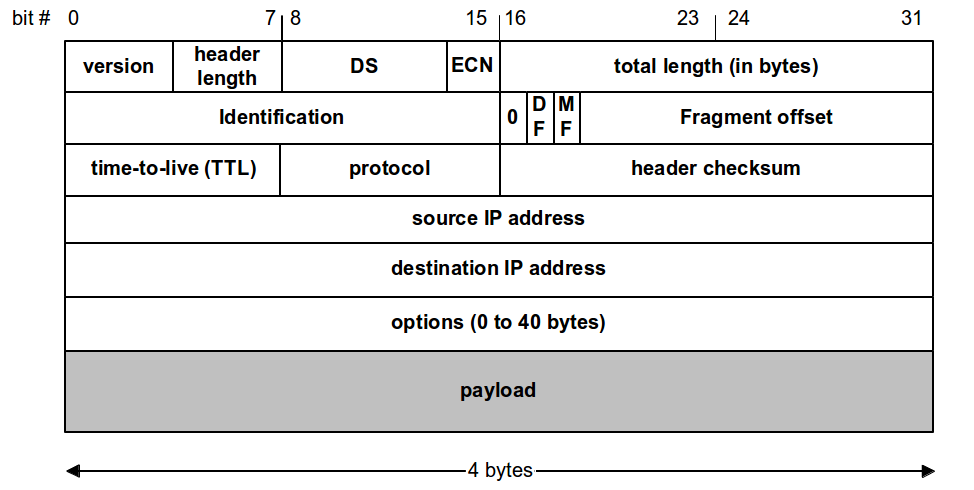
\includegraphics[width=1\textwidth]{ipDatagram.png}
 \caption[Paquete IP]{Paquete IP}
\end{figure}\par
Explicacion de los campos:\par
\begin{description}

\item[Version] representa la version del estándar actualmente es cuatro en transición a 6.
\item[Header Length] Tamaño del encabezado en múltiplos de 4 bytes.
\item[DS/ECN] Usado para especificar el nivel del servicio, actualmente no se usa y solo esta
presente para dar compatibilidad retroactiva.
\item[Identification] Identificación única del datagrama de un host, se incremente con cada 
datagrama.
\item[Flags] El primero siempre queda en cero, los otros dos indican si se fragmenta o tiene varios
fragmentos.
\item[TTL] Especifica la cantidad de caminos que puede tomar un paquete hasta que se lo descarte, se
utiliza para prevenir que el paquete quede para siempre dentro de un ciclo.
\item[Protocol] Especifica el numero del protocolo superior.
\item[Header Checksum] El checksum del header.
\item[Options] Restricciones de seguridad, registro de ruta(se agrega la dirección del router por el 
que pasa), marca de tiempo (por cada paso por router) y lista de rutas a pasar (por los únicos que 
puede pasar o por los que debe pasar entre otros)
\item[Padding] Se le agrega para asegurarse que tengo un tamaño de 4 bytes.

\end{description}


\section{El estándar IPv4}

\section{Porque abandonar IPv4}
Uno de los mayores problemas que presenta IPv4 es su tamaño, el cual ya ha quedado chico para los
estándares actuales. Este es un numero de solo 32bits con lo cual la cantidad máxima de números
posibles es $2^{32}$ cual da un total de 4.294.967.296 posibles dirección eso es menos de una
dirección por habitante\footnote{población actual de 7 mil millones de personas}.\par
Esto se ve mas limitante con la llegada masiva de los dispositivos mobiles, los cuales se conectan
a internet y la entrada de los grandes mercados emergentes del BRIC (Brasil, Rusia, India, China).
 
\section{La llegada de IPv6}
Principalmente internet era un prototipo que se hizo con un protocolo sencillo , nunca se creyo que tuvisese un crecimiento tan descomunal como para que en el futuro surgieran problemas tales como la seguridad entre el tráfico de datos a traves de la red , y la implementación de internet en otras tecnologías como  por ej celulares.Los problemas que hicieron inadecuada la version 4 de ip hicieron que se cambiara el sistema por completo por lo tanto los desarrolladores fueron forzados a crear un protocolo que resolviera los problemas actuales y trabajara diligentemente para asegurar que estos problemas no se encontraran nunca mas .Los desarrolladores del protocolo trabajaron diez años pero su implementación se hizo recientemente, es la implementación de un nuevo protocolo, escalable, ilimitado y con una gran proyeccion a futuro.\par

\section{Los Beneficios de IPv6}
Entre los principales beneficios de IPv6 fue la solucion a dos problemas fundamentales que tenia su protocolo antecesor: la falta de direcciones, y la escalabilidad de la ruta.Las soluciones implementadas fueron:
\begin{itemize}
\item Incremento de las direcciones IP
\item Desarrollo en la jerarquía de direcciones
\item Organización en los perfiles de red
\item Autoconfiguracion sencilla de la red
\item Mejora en la escalabilidad del enrutamiento
\item Enrutamiento a la mejor dirección posible(Anycast)
\item Mejoras en la seguridad
\item Mejoras en la movilidad
\item Se agregan nuevas tecnologías que mejoran la performance del protocolo

\end {itemize}
\begin{figure}[h!]
 \centering
 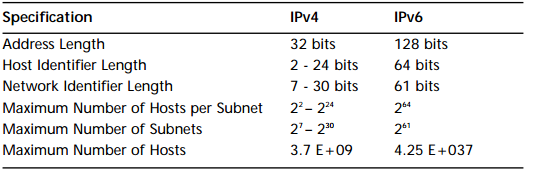
\includegraphics[width=1\textwidth]{comparativo_ip.png}
\end{figure} \par

\subsection{Jerarquía de Direcciones}
IPv6 divide las direcciones en distintos ambitos definidos o limites en los cuales se delegan las direcciones , por lo que soluciona problemas de disagregacion.Cuenta con un sistema de enrutamiento que permite discernir rapidamente el tipo de paquete que es, asi el enrutamiento se realiza de una forma mas sencilla y eficiente.
Otra de las herramientas que cabe destacar en IPv6 es el agregador de nivel superior \textbf{Top Level Aggregator (TLA)} que consta de dos propositos: el primero es la designacion de un gran bloque de direcciones compuesto por pequeños bloques que tienen la funcion de dar una conectividad descendiente a los que necesitan acceso a la red.El segundo es la detección de la ruta de origen,resulta mas claro ver quienes son los que tienen bloques de direcciones de proveedores y quienes son los que tienen una direccion local.Esto aumenta la eficiencia del nucleo de internet porque al agruparse de esta forma y haber una mejor organización de las direcciones , es mucho mas claro el pasaje de información.\par
Otro de los organismos existentes en este protocolo es el \textbf{NLA Next Level Aggregator} que si bien es demasiado pequeño para ser clasificado como un TDA , tiene una cadena principal regional extensa y cuenta con un numero de pequeños clientes.Sirve para dentro del gran bloque que proporciona el TDA , romper su porcion de direcciones y delegar las direcciones obtenidas a los \textbf{Sitios Agregadores de Servicio SLA}.Estos SLA se encargan de identificar subnets que no esten en el sitio.Otro beneficio importante que se puede destacar del NLA se relaciona con la estabilidad de ruta actual de todas las rutas a nivel mundial dejando de lado las inestabilidades conocidas como cortes,fallo en enlaces  y lentitud en el tráfico de datos.Debido a esta inestabilidad,  el concepto de "route dampening" surgió y trabaja de la siguiente forma: cada vez que una ruta se retira y se reanuncia , se le asigna una penalizacion que se mantiene hasta el lugar donde se encuentra la inestabilidad que por lo general suele ser una frontera exterior o  protocolo de puerta de enlace.Mientras mas alta sea la inestabilidad, mas alta será la penalidad asociada con la ruta.Cuando esa penalización alcanza cierto nivel, la ruta se retira y debe someterse a un período de espera.Mientras mas tiempo pasa , la pena va decreciendo hasta que la misma se disuelve y vuelve a estar permitida y se la reinserta en la tabla  de BGP del router.El propósito de esto es proveer una forma de negociar las inestabilidades de una forma tal que se minimice el costo de otros procesos que son importantes.\par
Cabe destacar que otro beneficio importante de la agregación la mejora importante en el enrutamiento, que forma parte de un requisito fundamental en IPv6.Así como hay mas direcciones tambien hay extensas ramificaciones y formas de organizarlas y controlarlas para que la asignacion de las mismas  no sea un problema.
\subsection{Un mecanismo de direccionamiento  mas sencillo}
El modelo IPv6 esta  caracterizado por tener  una direccion de 128.Los primeros 64 bits estan destinados a la numeracion de red y los ultimos 64 se utilizan para la numeracion del host, al tener 128 bits es mucho mas variada la cantidad de direcciones que se pueden formar  y tambien aumenta la seguridad de la red.Debemos recordar que los ultimos 64 btis del id del host se obtienen a partir de las direcciones mac de la red de interfaz.Por convencion la primera direccion se da normalmente al enrutador designado y el resto de las direcciones se asignan a los host de la subred con el ultimo domicilio.En IPv6 es un tanto diferente ya que  sabemos que la id es una direccion  de 64 bits que se obtiene de la direccion mac.Hoy en dia las direcciones MAC son de 48 bits , para llegar a 64 bits se las rellena con cadenas cadenas 0xff y 0xFE (: FF: FE: en términos IPv6) para cubrir la diferencia que existe entre la direccion MAC de la identificación de la companía y el ID proporcionado por el proveedor de la MAC.\par
El conflicto reside en si es necesario que las direcciones MAC tengan que cambiar su longitud  solo porque con el protocolo IPv6 cambia las longitudes del direccionamiento,si la necesidad de implementar direcciones MAC tan largas , la siguiente opcion para la longitud proporcionara mas de 1.8E019 direcciones mac en lugar de usar (264-248) si este viene a ser el
caso, simplemente puede dejar el relleno de la dirección MAC, y el uso de los 64 completo
bits de la dirección MAC para el ID de host
\subsection{Autoconfiguracion de direcciones}
La mejor ventaja de ipv6 sin dudas es la capacidad de autoconfiguracion de las direcciones ip.Antes de entrar en detalles sobre el tema hablaremos de \textbf{la direccion de multidifusion}.Esta consiste en una direccion multicast que se puede asignar simultaneamente a mas de una maquina.Esta direccion envia los paquetes al grupo de equipos asignados a la misma.Todas las maquinas que estan asignadas a esa direccion se dice que  estan en un grupo multicast,cuya direccion es la direccion  de multidifusion que utilizan.Los equipos conectados envian y reciben datos desde mas de un host.Se utiliza este estilo para realizar 1 a n o m transacciones.\par
Asociando este concepto con el de autoconfiguracion, se puede decir que una red lan es un grupo de maquinas y que cuando una nueva maquina ingresa a ese grupo , esta conectada y usan ipv6 , se le enviara a esa maquina nueva un paquete de multidifusion , este paquete se destinara a la  direccion de un ambito local.Cuando el router ve que este paquete entra , este se puede responder con la direccion de red de la maquina nueva .La respuesta recibe el paquete y a su vez , lee el numero de red que el router tiene enviado.Si se asigna una direccion de ipv6 añadiendo su ID de host.Todo este proceso no requiere ninguna intervencion manual por parte del administrador, esto asegura tambien la unicidad de la direccion , la maquina esta garantizada para tener la direccion unica , porque el numero de red exclusivamente asignado por el numero de router de esa red.
 Este mecanismo ahorra al usuario un monton de problemas tales como la configuracion manual cuando el equipo se mueve de una red a otra , la realizacion de un seguimiento de las direcciones que se ha asignado y cuales estan libres en un tiempo dado.
Esto le da una facilidad muy grande al administrador de redes ya que no debe perder tiempo en tareas de seguimiento y en el renombramiento de la red.\par
 \newpage
\subsection{Mejora en la Escalabilidad del Enrutamiento Multicast}


\section{Implementar IPv6}
\section{Desarrollo a futuro}

\newpage
\begin{thebibliography}{9}

\bibitem{redesTenem}
  Andrew S. Tanenbaum
  \emph{Redes de Computadoras}.
  USA,
  2003.

\bibitem{TaoIETF}
  Paul Hoffman
  \emph{The Tao of IETF: A Novice's Guide to the Internet Engineering Task Force}.
  USA,
  2012.
		
\bibitem{historyTCPiP}
  Gary C. Kessler
  \emph{An Overview of TCP/IP Protocols and the Internet}.
  USA,
  9 Nov 2010.
		
\bibitem{poolIPv4}
 nro.net
 \emph{Free Pool of IPv4 Address Space Depleted.} 
 19 Mar 2013\\
	\url{https://www.nro.net/news/ipv4-free-pool-depleted}	

\bibitem{IPv6 Architecture}

 \emph{Introduction to IPv6 Architecture} 

	\url{http://www.cu.ipv6tf.org/literatura/sample.pdf}		
		
\end{thebibliography}

\end{document}
